\chapter{Elementos de Cálculo Numérico}
\section{Soluções Numéricas}
\section{Diferenciação Numérica}

Vamos discutir nessa seção estratégias numéricas para aproximação de derivadas de funções reais. Nosso objetivo é calcular aproximadamente a derivada de uma função a partir de um conjunto de pontos discretos $\{(x_i,y_i)\}_{i=0}^n$. Começamos discutindo as chamadas aproximações por diferenças finitas e, então, as aproximações de derivadas via ajuste ou interpolação. 

Começamos com a fórmula mais simples que pode ser obtida do cálculo diferencial. Seja  uma função diferenciável $f: (a,b) \to \mathbb{R}$. A derivada de $f$  no ponto $x_0 \in (a,b)$  é, por definição,
\[ \frac{\dd }{\dd x} f(x_0) = \lim_{\delta \to 0} \frac{f(x_0+\delta) - f(x_0)}{\delta}.\]
Para aproximar a derivada podemos tomar $\delta > 0$ muito pequeno\footnote{Mesmo pequeno  $\delta$ ainda precisa ser muito maior do que a precisão de float-point, na verdade muito maior que a precisão númerica para o cálculo de $f(x)$, caso contrário corremos riscos de cancelamentos catastróficos.} e obter a aproximação:
\[\frac{\dd }{\dd x} f(x_0) \approx D^+_\delta f (x_0) = \frac{f(x_0+\delta) - f(x_0)}{\delta}  \]
que é chamada de {\it diferença finita progressiva de ordem 1}. De maneira similar temos a {\it diferença finita regressiva de ordem 1}, tomando $h<0$, ou de maneira análoga com $\delta>0$
\[\frac{\dd }{\dd x} f(x_0) \approx D^-_\delta f (x_0) = \frac{f(x_0) - f(x_0 - \delta)}{x_0}. \]
A existência da derivada de $f$ em $x_0$ garante que as duas aproximações tendam a um mesmo valor conforme $\delta \to 0$, i.e. 
\[ \lim_{\delta \to 0} |D_\delta^+ f(x_0) - D_\delta^- f(x_0) |= 0 \]

Vamos observar essa propriedade com a função cosseno em $\frac{\pi}{4}$ usando os valores
$\delta = 0.1, 10^{-2}, 10^{-3}, 10^{-4}$. 

\begin{lstlisting}
import numpy as np

def forward_dif(func, x, h):
    return (func(x+h) - func(x))/h

def regressive_dif(func, x, h):
    return (func(x) - func(x-h))/h

x =  np.pi/4
diferences = np.zeros(5)
h_list = [0.1, 0.01, 0.001, 0.0001, 0.00001]
for i,h in enumerate(h_list):
    diferences[i] = (forward_dif(np.cos, x , h)
                     - regressive_dif(np.cos, x , h))

print(diferences)
\end{lstlisting}

{\bf Exercício} adapte o código acima para calcular quão próximo estamos do valor correto da derivada de $\cos x$

Se $f$ for uma função analítica a obtenção de aproximações para derivadas é um consequência 
da expansão em série de Taylor
\[ f(x_0+\delta) = \sum_{k=1}^{+\infty} \frac{\dd^k}{\dd x^k}f(x_0) \frac{\delta^k}{k!},\]
onde $\frac{\dd^{0}}{\dd x^{0}} f(x_0) \equiv f(x_0)$. O erro ao truncarmos a expansão em um expoente $k=n+1$ é da ordem de $\delta^{n+1}$, mais precisamente
\[ f(x_0+\delta) = f(x_0) + \frac{\dd}{\dd x} f(x_0)\delta + \frac{\dd^2}{\dd x^2}f(x_0) \frac{\delta^2}{2} + \cdots + \frac{\dd^{k+1}}{\dd x^{k+1}}f(x_0) \frac{\delta^{k+1}}{n!}+\frac{\dd^k}{\dd x^k}f(\eta) \frac{\delta^k}{k!},\]
onde $\eta \in [x, x+\delta]$. Ou seja, nossa aproximação por diferenças finitas em primeira ordem possui um erro da ordem de $\delta^2$ (compare com o resultado do código acima). Podemos obter uma melhor aproximação fazendo um {\it diferença finita central}. Note que que
\[\begin{array}{rcl}
f(x_0+\delta) & = & f(x_0) + \frac{\dd}{\dd x}f(x_0) \delta + \frac{\dd^2}{\dd x^2}f(x_0)  \frac{\delta^2}{2!}+ \mathcal{O}(\delta^3)\\
f(x_0-\delta) & = & f(x_0) - \frac{\dd}{\dd x}f(x_0) \delta + \frac{\dd^2}{\dd x^2}f(x_0)  \frac{\delta^2}{2!}+ \mathcal{O}(\delta^3)
\end{array}\]
Temos portanto
\[f(x_0+\delta) - f(x_0-\delta) = 2 \frac{\dd}{\dd x}f(x_0) \delta + \mathcal{O}(\delta^3).\]
Com isso podemos adotar a aproximação
\[\frac{\dd }{\dd x} f(x_0) \approx D_\delta f (x_0) = \frac{f(x_0+\delta) - f(x_0-\delta)}{\delta}.\]

{\bf Exercício:} Mostre que $D_\delta f = D^+_\delta f - D^-_\delta f$

O exemplo abaixo utilizará as funções \lstinline{forward_dif} e \lstinline{regressive_dif} do exemplo anterior para compara os erros nas aproximações das derivadas de $f(x) = e^{e^x}$ em $x = 0$. O cálculo exato nos fornece (fazendo $u=e^x$)
\[f'(x) = \left.\frac{\dd e^u}{\dd u}\right|_{u=e^x} \left.\frac{\dd u}{\dd x}\right|_{x=0} = \left. e^{e^x}e^x \right|_{x=0} = e \]

\begin{lstlisting}[language = Python]
def center_dif(func, x, h):
    return (func(x+h) - func(x-h))/(2*h)

def exp_exp(x):
    return np.exp(np.exp(x))

e = np.exp(1)
Error_f = np.zeros(5)
Error_r = np.zeros(5)
Error_c = np.zeros(5)

h_list = [0.1, 0.01, 0.001, 0.0001, 0.00001]
for i,h in enumerate(h_list):
    Error_f[i] =  e - forward_dif(exp_exp, 0, h_list[i])
    Error_r[i] =  e - regressive_dif(exp_exp, 0, h_list[i])
    Error_c[i] = e - center_dif(exp_exp, 0, h_list[i])

print('Erro Progressivo=', Error_f, 'Erro regressivo', Error_r, 
    'Erro_central =', Error_c)
\end{lstlisting}

A série de Taylor também nos permite obter uma aproximação para a deriva segunda. Novamente
note que que
\[\begin{array}{rcl}
f(x_0+\delta) & = & f(x_0) + \frac{\dd}{\dd x}f(x_0) \delta + \frac{\dd^2}{\dd x^2}f(x_0)  \frac{\delta^2}{2!}+ \mathcal{O}(\delta^3)\\
f(x_0-\delta) & = & f(x_0) - \frac{\dd}{\dd x}f(x_0) \delta + \frac{\dd^2}{\dd x^2}f(x_0)  \frac{\delta^2}{2!}+ \mathcal{O}(\delta^3)
\end{array}\]
Temos portanto
\[f(x_0+\delta) + f(x_0-\delta) = 2 f(x_0) + \frac{\dd^2}{\dd x^2}f(x_0) +  \mathcal{O}(\delta^3).\]
E portanto podemos adotar a aproximação (com um erro da ordem de $\delta^2$)
\[\frac{\dd^2}{\dd x^2}f(x_0) \approx D_\delta^2 f(x_0) = \frac{f(x_0+\delta) + f(x_0-\delta) - 2 f(x_0)}{\delta^2}.\]

Vale destacar que existem outros métodos para aproximação de derivadas de uma função.

\subsection{Erros de Arredondamento}





\section{Integração Numérica}

\section{Equações Diferenciais Ordinárias}

Nessa Seção, vamos discutir métodos numéricos para aproximar a solução de problemas de valor inicial para equações diferenciais ordinárias. Com efeito toda a mecânica é um problema deste tipo. Por exemplo, considere uma força $F(x,\dot x, t)$ agindo em partícula que em $t=0$ esta na posição $x(0)=x_0$ e com velocidade $\dot x(0) = v_0$. Encontrar a posição e velocidade da partícula em um tempo $t>0$, consiste em encontrar uma função $x(t)$ que obedeça a equação diferencial de segunda ordem
\[ \ddot x = F(x,\dot x, t)\]
e satisfaça as condições iniciais $x(0)=x_0, \dot x(0) = v_0$.

Comecemos pelos problemas de primeira ordem e, depois, mostraremos que estas técnicas podem ser estendidas para problemas e sistemas de ordem superior. Considere um problema de valor inicial de primeira ordem dado por:

\begin{equation}\label{eq:1storderODE}\begin{array}{rcl}
\dot x(t) & = & f(x , t),\,\,\, t>0\\
x(t_0) & = & x_0
\end{array}\end{equation}

Vamos explorar como obter uma solução numérica para este problema. Vamos considerar inicialmente um método de passo único conhecido como método de Euler.

\subsection{Método de Euler}

Este é o método mais básico para integração numérica de equações diferenciais ordinárias. A ideia do método consiste em fixas um passo adequadamente pequeno $\Delta t$ e fazer a aproximação 
\[ \frac{\dd x(t)}{\dd t} \approx \frac{x(t+\Delta t) - x(t)}{\Delta t}\]
Dessa forma a eq \ref{eq:1storderODE} pode ser aproximada por
\begin{equation}\label{eq:Euler-Method}\begin{array}{rcl}
x(t + \Delta t) & = & x(t) + f(x , t) \Delta t + \mathcal{O}(\Delta t^2),\,\,\, t>0\\
x(t_0) & = & x_0.
\end{array}\end{equation}
Note que o erro da aproximação é da ordem de $\Delta t^2$.

Isso nos permite criar arrays com $N+1$ entradas
\[\begin{array}{rcl}
    t &=& [t_0, t_1, t_2, \cdots, t_N ] \\
    x &=& [x_0, x_1, x_2, \cdots, x_N ]
\end{array} \]
onde 
\[ t_{i+1} = t_i + \Delta t, \,\,\, x_{i+1} = x_i + f(x,t)\Delta t \]
e o passo $\Delta t = \left|\frac{t_N - t_0}{N} \right|$.

{\bf Exemplo:} Como um exemplo vamos considerar o caso 
\[\begin{array}{rcl}
\dot x(t) & = & x(t),\,\,\, t>0\\
x(0) & = & 1
\end{array}\]
Este problema tem uma solução analítica simples dada por $x(t)=e^{t}$ que pode ser verificada diretamente por substituição na EDO acima. 

\begin{lstlisting}[language = Python]
import numpy as np
import matplotlib.pyplot as plt

tempo_0 = 0
tempo_f = 1
x_0 = 1
passos = 1000
dt = (tempo_f - tempo_0)/passos
t_list = np.zeros(passos)
x_list = np.zeros(passos)

#Condicoes iniciais
t_list[0] = tempo_0
x_list[0] = x_0

for i in range(passos-1):
    t_list[i+1] =  t_list[i]+dt
    x_list[i+1] = x_list[i]*(1+dt)

plt.scatter(t_list, x_list, label='Metodo de Euler', marker='+')
plt.plot(t_list, np.exp(t_list), 
    label='Resultado Analitico', color='red')
plt.legend()
plt.show()
print('Tamanho do passo=', dt, 'Erro Maximo =', 
    np.abs((x_list-np.exp(t_list))).max())
\end{lstlisting}

Varie o tamanho do passo e note oque acontece com o erro.

{\bf Exemplo:} Vamos considerar agora o caso
\[\begin{array}{rcl}
\dot x(t) & = & \cos t,\,\,\, t>0\\
x(0) & = & 0
\end{array}\]
É fácil ver que a solução deste problema é dada por $x(t) = \sin t$. Nesse exemplo vemos como a ordem de escolha do valor de $t$ para o update da posição $x$ é relevante. Note que temos duas formas:
\[ x(t+dt) \approx x(t) = dt*\cos t,\,\, \textrm{e} \,\,\,x(t+dt) \approx x(t) = dt*\cos (t+dt)\]

Na primeira utilizamos o valor anterior de $t$ para o cálculo da derivada e enquanto no segundo caso utilizamos o valor $t+dt$ para o cálculo da derivada.


\begin{lstlisting}[language = Python]
import numpy as np
import matplotlib.pyplot as plt

tempo_0 = 0
tempo_f = 3
x_0 = 0
passos = 100
dt = (tempo_f - tempo_0)/passos
t_list = np.zeros(passos)
x_list = np.zeros(passos)
x_list1 = np.zeros(passos)

#Condicoes iniciais
t_list[0] = tempo_0
x_list[0] = x_0

for i in range(passos-1):
    t_list[i+1] =  t_list[i]+dt
    x_list[i+1] = x_list[i]+np.cos(t_list[i])*dt
    x_list1[i+1] = x_list1[i]+np.cos(t_list[i+1])*dt

plt.scatter(t_list, x_list, label='Metodo de Euler update c\ t anterior', 
    marker='+', s=1)
plt.scatter(t_list, x_list1, label='Metodo de Euler update c\ t atual',
    marker='o', s=1)
plt.plot(t_list, np.sin(t_list), label='Solucao Analitica',
    color='red', linewidth=0.5)
plt.legend()
plt.show()
print('Tamanho do passo=', dt, 'Erro Maximo (t anterior)=', np.abs((x_list-np.sin(t_list))).max(),
     'Erro Maximo (t atual)=', np.abs((x_list1-np.sin(t_list))).max())
\end{lstlisting}

A saída deve ser como a mostrada na 

\begin{figure}
    \centering
    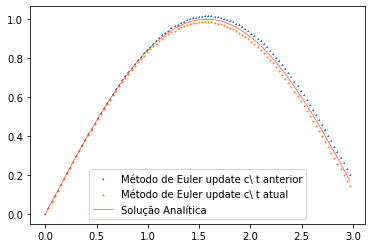
\includegraphics{Images/euler2.png}
    \caption{Método de Euler progressivo e Regressivo}
    \label{fig:euler2}
\end{figure}

\subsection{Variações do Método de Euler}
\subsection{Método de Runge-Kutta}
\section{Método de Monte Carlos}\label{sc:Monte_Carlo}
\section{Métodos Estocásticos}
\section{Equações Diferenciais Parciais}
\subsection{Equação de Laplace}
\subsection{Equação da Onda}
\subsection{Equação do Calor}
